% Seperti yang telah dijelaskan pada \ref{sec:alternatif-solusi}, solusi yang dipilih adalah dengan mengkombinasikan antara sistem \textit{in-memory key-value store} milik Memcache dan menggunakan \textit{database} terpisah sebagai tempat penyimpanan data \textit{persistence}. Replikasi dan \textit{erasure coding} dapat dilakukan pada data persisten yang disimpan pada \textit{database} tersebut. Adapun gambaran umum arsitektur sistem dapat dilihat pada gambar \ref{fig:general-architecture}

Seperti yang telah dijelaskan pada \ref{sec:alternatif-solusi}, solusi yang dipilih adalah membuat sistem dengan mengkombinasikan Memcached sebagai \textit{in-memory key-value store} dan menggunakan RocksDB sebagai \textit{persistent database}. Replikasi dan \textit{erasure coding} hanya dilakukan pada data persisten yang disimpan pada \textit{database} tersebut. Dari sistem tersebut, komponen yang perlu dikembangkan adalah
\begin{enumerate}
  \item \textbf{Database Node} yang merupakan integrasi dari Memcached dan RocksDB. Berperan juga untuk menerima \textit{request} dari \textit{client} dan tempat dilaksanakannya operasi dengan \textit{erasure coding} maupun replikasi.
  \item \textbf{Erasure Coding Module} yang dapat meng-\textit{encode} dan \textit{decode} data dengan \textit{erasure coding} pada \textit{node}.
  \item \textbf{Client} yang dapat mengumpulkan data serta memvariasikan faktor-faktor sesuai kebutuhan eksperimen.
\end{enumerate}

Selain itu, pengembangan akan dilakukan dengan menggunakan bahasa pemrograman Rust karena Rust merupakan bahasa sistem berkinerja tinggi. Selain itu, Rust sudah memiliki \textit{support} untuk semua kakas yang dibutuhkan. Pengembangan akan memanfaatkan pustaka yang ada untuk mempermudah pengembangan. Penjelasan detail mengenai modul-modul tersebut dapat dilihat pada lampiran a.

Eksperimen ini dijalankan dengan \textit{client} mengirimkan \textit{request} ke \textit{database node} untuk melakukan operasi tertentu. Kemudian \textit{database node} akan melakukan operasi yang diminta. Setelah itu, \textit{database node} dapat melakukan \textit{erasure coding} sesuai konfigurasi dan mendistribusikan data yang diterima. Penjelasan detail mengenai flow terdapat pada lampiran b. Selain itu, gambaran umum arsitektur sistem dapat dilihat pada lampiran c

\ref{fig:general-architecture}.
  
% TODO: Penjelasan Modul, pindahkan gambar ke lampiran
\begin{figure}[ht]
    \centering
    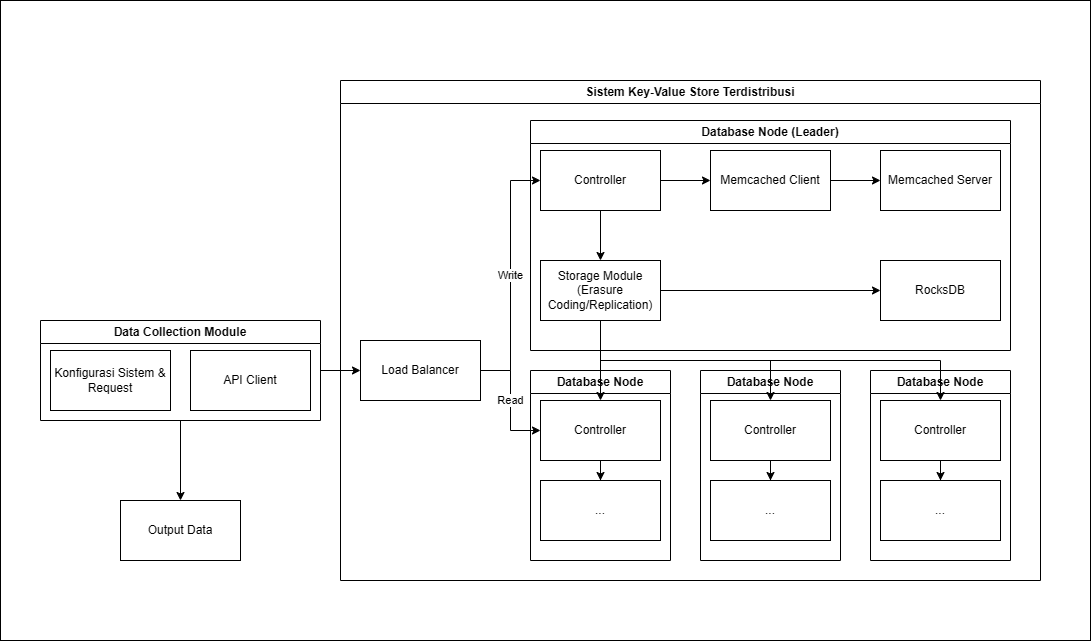
\includegraphics[width=0.95\textwidth]{resources/chapter-3/general-architecture.png}
    \caption{Gambaran Umum Arsitektur Sistem Eksperimen}
    \label{fig:general-architecture}
  \end{figure}